\documentclass[border=3pt]{standalone}
% Preâmbulo compartilhado pelos diagramas TikZ da aula 10 de IHC (Planejamento da Avaliação)
\usepackage[T1]{fontenc}
\usepackage[utf8]{inputenc}
\usepackage{lmodern}
\usepackage{amsmath}
\usepackage{xcolor}
\usepackage{tikz}
\usetikzlibrary{arrows.meta,angles,quotes,decorations.pathmorphing,decorations.pathreplacing,calc,
                positioning,shapes.geometric,shapes.misc,backgrounds,fit,
                math}

% Paleta (mesma dos SVGs originais)
% Paleta da disciplina de IHC: acento roxo (#755099), da capa do livro.
% (o nome "dblue" é mantido para não alterar todos os diagramas)
\definecolor{dblue}{HTML}{755099}
\definecolor{dorange}{HTML}{B3541E}
\definecolor{dgreen}{HTML}{4A7C59}
\definecolor{dred}{HTML}{9C4B4B}
\definecolor{dcream}{HTML}{F4F1EA}
\definecolor{dshade}{HTML}{DDD7C9}

% Função gaussiana (não normalizada por padrão de escala visual)
\pgfmathdeclarefunction{gauss}{3}{%
  \pgfmathparse{1/(#3*sqrt(2*pi))*exp(-((#1-#2)^2)/(2*#3^2))}%
}

% Estilos comuns (prefixo d... para não colidir com chaves internas do pgf)
\tikzset{
  >={Stealth[length=2mm]},
  dguide/.style={gray!55, dashed, line width=0.4pt},
  daxis/.style={gray!60, line width=0.7pt, ->},
  dbody/.style={fill=black!3, draw=black!80, line width=1pt},
  dacc/.style={draw=dblue, line width=1pt},
  dlbl/.style={black!55, font=\small},
  dsub/.style={black!45, font=\footnotesize},
  dstate/.style={circle, draw=black!80, fill=dcream, line width=1pt,
                 minimum size=17mm, font=\large, inner sep=1pt},
  dobs/.style={circle, draw=black!80, fill=dshade, line width=1pt,
               minimum size=14mm, font=\large, inner sep=1pt},
  dbox/.style={rounded corners=2pt, draw=black!80, fill=dcream, line width=1pt,
               align=center, inner sep=6pt},
  dop/.style={circle, draw=black!80, fill=white, line width=1pt,
              minimum size=6mm, inner sep=0pt, font=\small},
  dtrans/.style={->, dblue, line width=1pt},
  dmeas/.style={->, dorange, line width=1pt},
  dcurve/.style={line width=1pt, dblue},
  dcurveb/.style={line width=1.4pt, dorange},
}

\begin{document}
\hyphenpenalty=10000 \exhyphenpenalty=10000 \tolerance=9999 \emergencystretch=3em
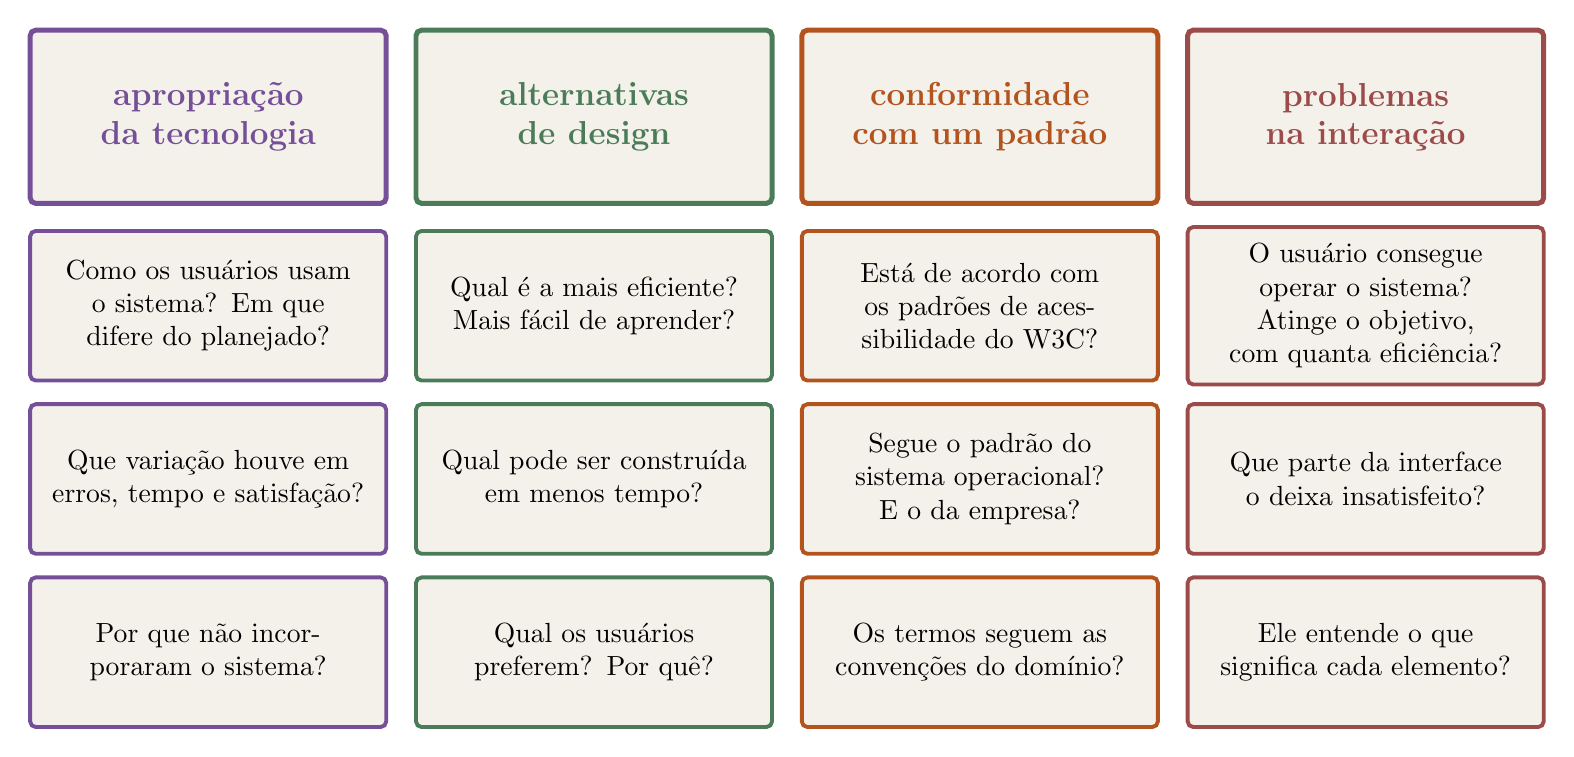
\begin{tikzpicture}[x=1cm,y=1cm]
\tikzset{h/.style={dbox, text width=4.1cm, minimum height=2.2cm, font=\large\bfseries, line width=1.8pt},
        q/.style={dbox, text width=4.1cm, minimum height=1.9cm, font=\normalsize, line width=1.4pt}}
\node[h, draw=dblue] at (2.2,7.0) {\textcolor{dblue}{apropriação da tecnologia}};
\node[q, draw=dblue] at (2.2,4.6) {Como os usuários usam o sistema? Em que difere do planejado?};
\node[q, draw=dblue] at (2.2,2.4) {Que variação houve em erros, tempo e satisfação?};
\node[q, draw=dblue] at (2.2,0.2) {Por que não incorporaram o sistema?};
\node[h, draw=dgreen] at (7.1,7.0) {\textcolor{dgreen}{alternativas de design}};
\node[q, draw=dgreen] at (7.1,4.6) {Qual é a mais eficiente? Mais fácil de aprender?};
\node[q, draw=dgreen] at (7.1,2.4) {Qual pode ser construída em menos tempo?};
\node[q, draw=dgreen] at (7.1,0.2) {Qual os usuários preferem? Por quê?};
\node[h, draw=dorange] at (12.0,7.0) {\textcolor{dorange}{conformidade com um padrão}};
\node[q, draw=dorange] at (12.0,4.6) {Está de acordo com os padrões de acessibilidade do W3C?};
\node[q, draw=dorange] at (12.0,2.4) {Segue o padrão do sistema operacional? E o da empresa?};
\node[q, draw=dorange] at (12.0,0.2) {Os termos seguem as convenções do domínio?};
\node[h, draw=dred] at (16.9,7.0) {\textcolor{dred}{problemas na interação}};
\node[q, draw=dred] at (16.9,4.6) {O usuário consegue operar o sistema? Atinge o objetivo, com quanta eficiência?};
\node[q, draw=dred] at (16.9,2.4) {Que parte da interface o deixa insatisfeito?};
\node[q, draw=dred] at (16.9,0.2) {Ele entende o que significa cada elemento?};
\end{tikzpicture}
\end{document}
